\documentclass[spec, och, labwork]{shiza}
% параметр - тип обучения - одно из значений:
%    spec     - специальность
%    bachelor - бакалавриат (по умолчанию)
%    master   - магистратура
% параметр - форма обучения - одно из значений:
%    och   - очное (по умолчанию)
%    zaoch - заочное
% параметр - тип работы - одно из значений:
%    referat    - реферат
%    coursework - курсовая работа (по умолчанию)
%    diploma    - дипломная работа
%    pract      - отчет по практике
% параметр - включение шрифта
%    times    - включение шрифта Times New Roman (если установлен)
%               по умолчанию выключен
\usepackage{subfigure}
\usepackage{tikz,pgfplots}
\pgfplotsset{compat=1.5}
\usepackage{float}

%\usepackage{titlesec}
\setcounter{secnumdepth}{4}
%\titleformat{\paragraph}
%{\normalfont\normalsize}{\theparagraph}{1em}{}
%\titlespacing*{\paragraph}
%{35.5pt}{3.25ex plus 1ex minus .2ex}{1.5ex plus .2ex}

\titleformat{\paragraph}[block]
{\hspace{1.25cm}\normalfont}
{\theparagraph}{1ex}{}
\titlespacing{\paragraph}
{0cm}{2ex plus 1ex minus .2ex}{.4ex plus.2ex}

% --------------------------------------------------------------------------%


\usepackage[T2A]{fontenc}
\usepackage[utf8]{inputenc}
\usepackage{graphicx}
\graphicspath{ {./images/} }
\usepackage{tempora}

\usepackage[sort,compress]{cite}
\usepackage{amsmath}
\usepackage{amssymb}
\usepackage{amsthm}
\usepackage{fancyvrb}
\usepackage{listings}
\usepackage{listingsutf8}
\usepackage{longtable}
\usepackage{array}
\usepackage[english,russian]{babel}

% \usepackage[colorlinks=true]{hyperref}
\usepackage{url}

\usepackage{underscore}
\usepackage{setspace}
\usepackage{indentfirst} 
\usepackage{mathtools}
\usepackage{amsfonts}
\usepackage{enumitem}
\usepackage{tikz}
\usepackage{minted}

\newcommand{\eqdef}{\stackrel {\rm def}{=}}
\newcommand{\specialcell}[2][c]{%
\begin{tabular}[#1]{@{}c@{}}#2\end{tabular}}

\renewcommand\theFancyVerbLine{\small\arabic{FancyVerbLine}}

\newtheorem{lem}{Лемма}

\begin{document}

% Кафедра (в родительном падеже)
\chair{}

% Тема работы
\title{Алгоритм дерева бинарного поиска}

% Курс
\course{3}

% Группа
\group{331}

% Факультет (в родительном падеже) (по умолчанию "факультета КНиИТ")
\department{факультета КНиИТ}

% Специальность/направление код - наименование
%\napravlenie{09.03.04 "--- Программная инженерия}
%\napravlenie{010500 "--- Математическое обеспечение и администрирование информационных систем}
%\napravlenie{230100 "--- Информатика и вычислительная техника}
%\napravlenie{231000 "--- Программная инженерия}
\napravlenie{100501 "--- Компьютерная безопасность}

% Для студентки. Для работы студента следующая команда не нужна.
% \studenttitle{Студентки}

% Фамилия, имя, отчество в родительном падеже
\author{Окунькова Сергея Викторовича}

% Заведующий кафедрой
% \chtitle{} % степень, звание
% \chname{}

%Научный руководитель (для реферата преподаватель проверяющий работу)
\satitle{доцент} %должность, степень, звание
\saname{А. Н. Гамова}

% Руководитель практики от организации (только для практики,
% для остальных типов работ не используется)
% \patitle{к.ф.-м.н.}
% \paname{С.~В.~Миронов}

% Семестр (только для практики, для остальных
% типов работ не используется)
%\term{8}

% Наименование практики (только для практики, для остальных
% типов работ не используется)
%\practtype{преддипломная}

% Продолжительность практики (количество недель) (только для практики,
% для остальных типов работ не используется)
%\duration{4}

% Даты начала и окончания практики (только для практики, для остальных
% типов работ не используется)
%\practStart{30.04.2019}
%\practFinish{27.05.2019}

% Год выполнения отчета
\date{2022}

\maketitle

% Включение нумерации рисунков, формул и таблиц по разделам
% (по умолчанию - нумерация сквозная)
% (допускается оба вида нумерации)
% \secNumbering

%-------------------------------------------------------------------------------------------
\tableofcontents

\section{Описание алгоритма}

Бинарное дерево — это иерархическая структура данных, в которой каждый узел имеет значение 
(оно же является в данном случае и ключом) и ссылки на левого и правого потомка. Узел, 
находящийся на самом верхнем уровне (не являющийся чьим либо потомком) называется корнем. 
Узлы, не имеющие потомков (оба потомка которых равны NULL) называются листьями.статком данного 
алгоритма.

Бинарное дерево поиска — это бинарное дерево, обладающее дополнительными свойствами: значение 
левого потомка меньше значения родителя, а значение правого потомка больше значения родителя 
для каждого узла дерева. То есть, данные в бинарном дереве поиска хранятся в отсортированном виде. 
При каждой операции вставки нового или удаления существующего узла отсортированный порядок дерева 
сохраняется. При поиске элемента сравнивается искомое значение с корнем. Если искомое больше корня, 
то поиск продолжается в правом потомке корня, если меньше, то в левом, если равно, то значение найдено 
и поиск прекращается.

\section{Эффективность алгоритма}

Так как для добавления элемента в дерево бинарного поиска нам не нужно проходить все дерево, а нужно только
найти элемент, для которого мы определим его как потомка, то операция вставки в бинарное дерево поиска имеет 
сложность $O(\log n)$, где n - размер дерева.

Чтобы создать дерево из массива, нужно n раз вызвать операцию вставки в дерево. Из всего выше сказанного очевидно, 
что вычислительная сложность создания дерева бинарного поиска определяется как $O(n\log n)$.

За счет свойств дерева бинарного поиска сам  поиск работает по такому принципу, что на каждом шаге мы спускаемся 
на один уровень дерева вниз. Очевидно что в худшем случае рекурсия пройдет по всем уровням, колличество которых
равняется $\log_2 n$. Отсюда следует, что вычислительная сложность поиска определяется как $O(\log n)$.

\section{Реализация}

    \inputminted[fontsize=\small]{py}{lab2.py}

    \section{Тестирование программы}

    \begin{figure}[H]
        \centering      %размер рисунка       здесь находится название файла рисунка, без указания формата
        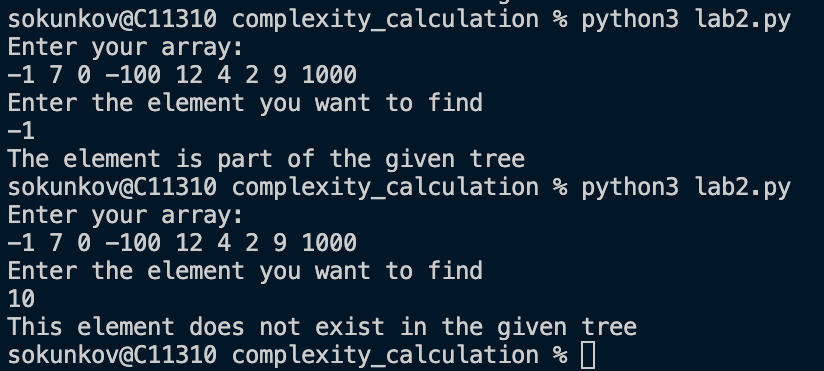
\includegraphics[width=1.\textwidth]{2}
        \caption{Тест1}
        \label{fig:image1}
    \end{figure}
    
    \newpage
    
    \begin{thebibliography}{3}
        \bibitem{1}
        Скиена Стивен "Алгоритмы. Руководство по разработке", 2018 год. Яз. рус.
        \bibitem{2}
        Нииколаус Вирт "Алгоритмы и структуры данных", 2008 год. Яз. рус.
    \end{thebibliography}

\end{document}